\documentclass[10pt,a4paper,twocolumn]{article}
\usepackage{iftex}
\ifPDFTeX\input{glyphtounicode}\pdfgentounicode=1\fi
\usepackage[T1]{fontenc}
\usepackage{newtxtext,newtxmath,microtype}
\usepackage[top=20mm,bottom=20mm,left=18mm,right=18mm,columnsep=7mm]{geometry}
\usepackage{graphicx,booktabs,tabularx,array,amsmath,tikz,caption,titlesec}
\usetikzlibrary{arrows.meta,positioning}
\usepackage{cite,balance,xurl}
\usepackage[hidelinks]{hyperref}
\hypersetup{pdftitle={Core Explorer: Design, Implementation, and Evaluation of a Voxel-Based Platform Game},pdfauthor={Jacky Hui (Member A) and Jerry Xie (Member B)}}
\graphicspath{{images/}}
\pagestyle{plain}
\raggedbottom
\clubpenalty=10000
\widowpenalty=10000
\displaywidowpenalty=10000
\setlength{\emergencystretch}{1em}
\urlstyle{same}
\setlength{\parindent}{1em}
\setlength{\parskip}{0pt}
\setlength{\tabcolsep}{4pt}
\renewcommand{\arraystretch}{1.1}
\setlength{\textfloatsep}{10pt plus 2pt minus 2pt}
\setlength{\dbltextfloatsep}{10pt plus 2pt minus 2pt}
\setlength{\floatsep}{8pt plus 2pt minus 2pt}
\setlength{\dblfloatsep}{8pt plus 2pt minus 2pt}
\renewcommand{\topfraction}{.9}
\renewcommand{\dbltopfraction}{.9}
\renewcommand{\textfraction}{.08}
\renewcommand{\floatpagefraction}{.85}
\renewcommand{\dblfloatpagefraction}{.85}
\setcounter{topnumber}{3}
\setcounter{dbltopnumber}{3}
\captionsetup{font=small,labelfont=bf,labelsep=period,skip=4pt,hypcap=false}
\titleformat{\section}{\normalfont\large\bfseries}{\thesection.}{.55em}{}
\titleformat{\subsection}{\normalfont\normalsize\bfseries}{\thesubsection}{.55em}{}
\titlespacing*{\section}{0pt}{10pt plus 2pt minus 2pt}{5pt}
\titlespacing*{\subsection}{0pt}{7pt plus 1pt minus 1pt}{3pt}
\newcommand{\code}[1]{\texttt{#1}}
\newcommand{\shot}[2]{\begin{minipage}[t]{.485\linewidth}\centering\includegraphics[width=\linewidth]{#1}\par{\small #2}\end{minipage}}
\begin{document}
\twocolumn[
\begin{@twocolumnfalse}
\begin{center}
{\LARGE\bfseries Core Explorer: Design, Implementation, and\\[2pt]
Evaluation of a Voxel-Based Platform Game\par}
\vspace{7pt}
{\large Jacky Hui (Member A) \qquad Jerry Xie (Member B)\par}
\end{center}
\begin{abstract}
This report presents the design and evaluation of Core Explorer, a third-person voxel platform game implemented in C++17 and OpenGL 3.3 Core. A $96^3$ voxel representation supports an untimed training environment and two missions with different navigation and movement demands. The implementation combines hierarchical robot and gate models, world-space Blinn--Phong lighting, procedural normal maps and a bounded event-driven particle system. Hidden-face removal is evaluated against a baseline that submits all voxel faces. At a $1920\times1080$ framebuffer resolution, with 60 warm-up frames and 240 measured frames per run, the optimisation reduces mean scene-rendering time by 8.1--19.7\% across the three configurations on an RTX 4060 Laptop GPU. The results demonstrate a reduction in geometry cost without changing draw-call counts. Remaining map/test inconsistencies and unverified VLAB/CSE execution limit conclusions about end-to-end gameplay completeness and platform portability.
\end{abstract}
\vspace{2pt}
\noindent\textbf{Keywords:} voxel rendering; hierarchical modelling; normal mapping; particle systems; performance evaluation.
\vspace{12pt}
\end{@twocolumnfalse}
]
\section{Introduction and Game Design}\label{sec:design}
Core Explorer is a single-player, third-person voxel platform game. A repair robot collects every energy core in a facility and reaches the unlocked exit. Its three authored environments combine spatial navigation, timed hazards and physical interactions. The training yard introduces the mechanisms; the two missions place different demands on route planning and movement precision.

\begin{table*}[t]
\centering
\caption{Authored configurations and gameplay objectives. Dimensions denote horizontal room extents.}\label{tab:levels}
\small
\begin{tabularx}{\linewidth}{@{}l l X@{}}
\toprule
\textbf{Configuration} & \textbf{Current layout} & \textbf{Objective and distinguishing mechanics}\\
\midrule
Tutorial Yard & $32\times32$, 3 cores & Untimed; crawl passage, relay-controlled shock floor, moving obstacle, ground/upper doors, jump pad and portal pair.\\
Helios Yard & $84\times60$, 4 cores & 600 seconds; four districts with rooftop access, electric-floor traversal and layered/corridor mazes; five pressure-plate doors and one portal pair.\\
Corona Run & $76\times76$, 9 cores & 300 seconds; elevated parkour above a hazardous red floor, narrow beams, gaps and moving obstacles; four checkpoints and four jump pads, without portals.\\
\bottomrule
\end{tabularx}
\end{table*}

\par\vspace{2mm}
These are horizontal room dimensions, not the storage volume: every configuration uses a $96\times96\times96$ voxel world, including empty cells. Table~\ref{tab:levels} describes the evaluated level files. The two missions are shown in Figure~\ref{fig:levels}.

\begin{figure*}[t]
\centering
\shot{helios.png}{(a) Helios Yard: districts and mechanisms}\hfill
\shot{corona.png}{(b) Corona Run: elevated routes over the void}
\caption{Current mission configurations, captured in the whole-room overview. The HUD shows armour, remaining lives, time and the required core slots.}\label{fig:levels}
\end{figure*}

\subsection{Controls and rules}
\textbf{WASD} moves relative to the camera; \textbf{mouse} orbits and the \textbf{wheel} changes distance. \textbf{Shift} sprints, \textbf{Space} jumps, \textbf{C} toggles crouching and \textbf{E} interacts with cores, relays and portal endpoints. Checkpoints save automatically when reached. \textbf{R} restarts, \textbf{Esc} pauses, and \textbf{V} toggles a north-up orthographic surveillance view with map-relative movement. Bindings are configurable in Settings. The minimap supports navigation in the follow view.

The robot has five armour units. Falling onto the void floor costs one armour unit and returns the robot to its checkpoint. Damage has a cooldown; loss of all armour triggers a 2.2-second reboot at the last checkpoint or entry. Timed missions allow three lives; ordinary reboots retain collected cores and elapsed time, restore armour and grant one second of protection. Exhausting lives restarts the mission; reaching the time limit fails the run. Training has unlimited time and lives. Relays temporarily disable linked shock plates, pressure plates unlock doors, and jump pads launch the robot automatically. Pauses and level-transition holds stop the gameplay clock.


\section{System Architecture}\label{sec:system}
\subsection{World, state and collision}
\code{LevelData} parses text files into material-valued cells and typed mechanisms; \code{Game} owns the voxel world, player, timers, hazards, interaction state and particles. The main loop separates title/play/pause/settings screens and level transitions from the simulation states Playing/Won/Lost. A reset reconstructs the chosen configuration and clears transient state. Simulation advances in substeps of at most $1/120$ second. A vertical player cylinder is tested against occupied voxel boxes, moving-hazard parts and mechanism fixtures; movement is resolved by axis, with crouch clearance checked before standing. Render-only limb motion does not change the collision body.

\subsection{Geometry and rendering}
C++17 and OpenGL 3.3 Core render true 3D geometry with a depth buffer. Terrain is generated as UV-mapped triangle faces; shared boxes, spheres and cylinders form the robot and mechanisms. Model instances are grouped by primitive and blend mode. \code{Renderer::}\allowbreak\code{prepare} builds/uploads geometry and instances; \code{draw} applies the camera, GLSL materials and scene effects. Framebuffer dimensions drive the viewport and projection. The procedural star background uses a fullscreen triangle reconstructed from viewing directions; it uses no sky image. F1 displays live geometry and camera diagnostics (Figure~\ref{fig:diagnostics}).

\begin{figure*}[t]
\centering
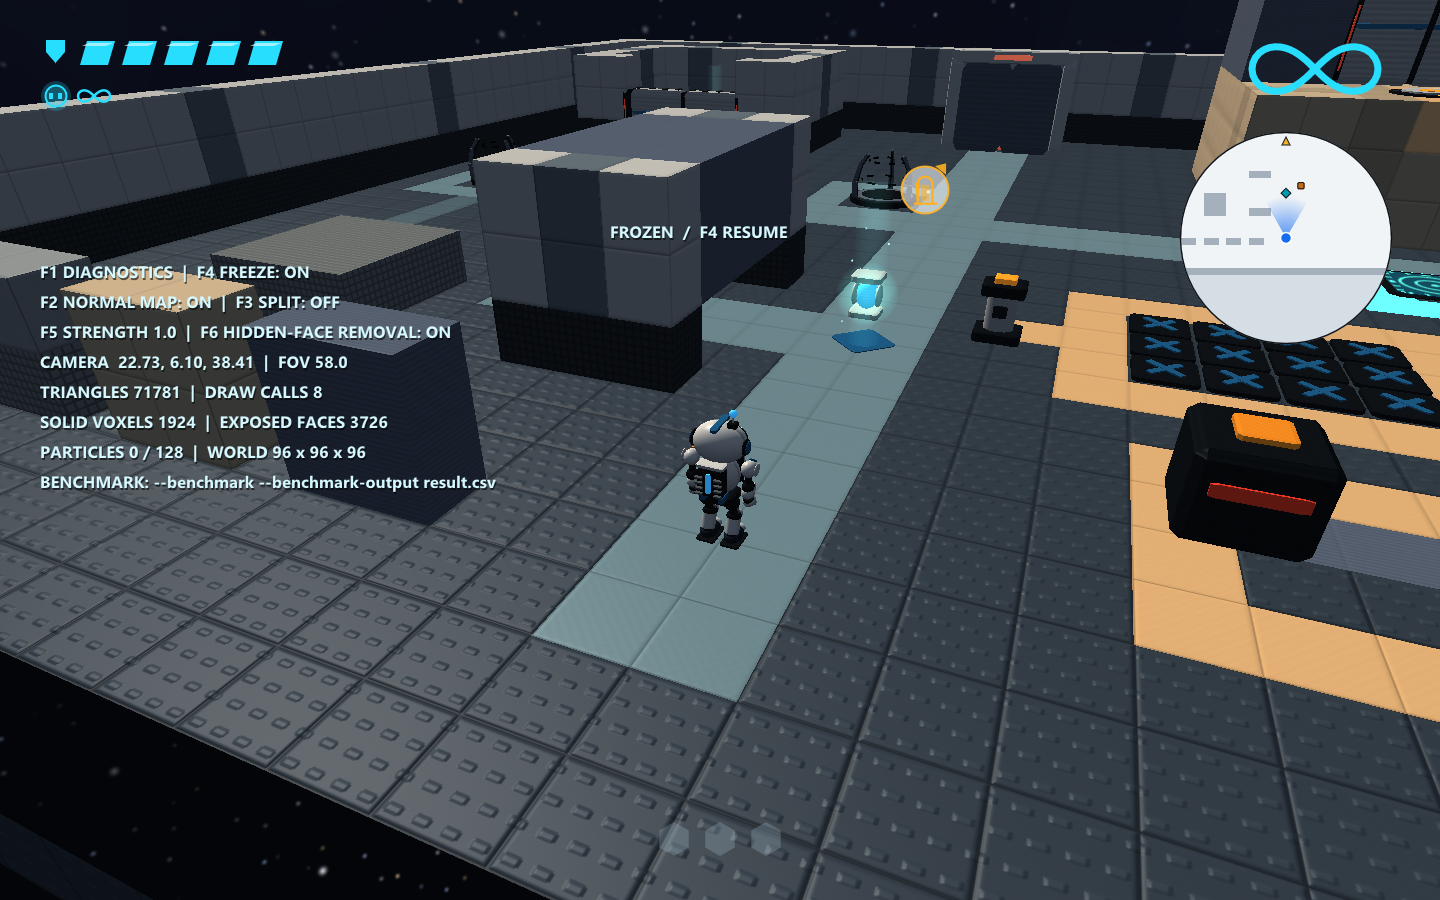
\includegraphics[width=.85\linewidth,trim=0bp 130bp 80bp 170bp,clip]{perspective-diagnostics.png}
\caption{Perspective scene with live diagnostics: 71,781 submitted triangles, eight draw calls, 1,924 solid voxels and 3,726 exposed faces. Camera position is $(22.73,6.10,38.41)$ with a $58^\circ$ vertical field of view. The screenshot is cropped to emphasise scene geometry and the diagnostic overlay.}\label{fig:diagnostics}
\end{figure*}

\subsection{Two multipart hierarchies}
For node $i$, the inherited joint matrix is $J_i=J_{p(i)}T_iR_{x,i}R_{y,i}R_{z,i}$; a root uses the object's world transform. Its drawn mesh uses $M_i=J_iS_i$. Keeping mesh dimensions out of the inherited joint transform prevents a scaled torso from stretching the arms. The robot's root handles world motion/yaw, while children supply gait and reaction poses. The exit gate has a separate root and independently translating panels (Figure~\ref{fig:hierarchy}); handles and stripes follow their parent panel.

\begin{figure*}[t]
\centering
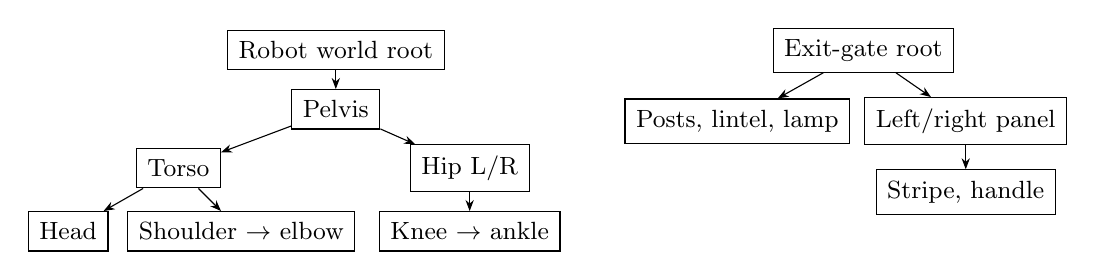
\begin{tikzpicture}[font=\small,box/.style={draw=black,fill=white,inner sep=4pt,align=center},edge/.style={-{Stealth[length=1.4mm]},thin},x=1cm,y=1cm]
\node[box] (r) at (0,0) {Robot world root};
\node[box] (p) at (0,-.75) {Pelvis};
\node[box] (t) at (-2,-1.5) {Torso};
\node[box] (h) at (1.7,-1.5) {Hip L/R};
\node[box] (head) at (-3.4,-2.3) {Head};
\node[box] (arm) at (-1.2,-2.3) {Shoulder $\to$ elbow};
\node[box] (leg) at (1.7,-2.3) {Knee $\to$ ankle};
\draw[edge] (r)--(p);\draw[edge] (p)--(t);\draw[edge] (p)--(h);
\draw[edge] (t)--(head);\draw[edge] (t)--(arm);\draw[edge] (h)--(leg);
\node[box] (g) at (6.7,0) {Exit-gate root};
\node[box] (f) at (5.1,-.9) {Posts, lintel, lamp};
\node[box] (d) at (8,-.9) {Left/right panel};
\node[box] (s) at (8,-1.8) {Stripe, handle};
\draw[edge] (g)--(f);\draw[edge] (g)--(d);\draw[edge] (d)--(s);
\end{tikzpicture}
\caption{Simplified parent-child graph of the two textured articulated models. Each left/right branch is instantiated separately.}\label{fig:hierarchy}
\end{figure*}


\section{Surface Shading and Normal Mapping}\label{sec:normal}
\subsection{Lighting model and material differentiation}
The shader uses world-space positions and view/light directions. Geometric normals are transformed by the inverse transpose of the model matrix. The opaque surface colour combines hemispheric ambient light, Lambert diffuse, Blinn--Phong specular, emission and distance fog:
\begin{equation}
\begin{aligned}
C &= a\bigl(A + L_d\max(0,n\!\cdot\!l)\bigr)\\
  &\quad + L_s k_s\max(0,n\!\cdot\!h)^p + E,\\
h &= \frac{l+v}{\|l+v\|}.
\end{aligned}
\label{eq:lighting}
\end{equation}
The implementation generates five periodic $64\times64$ albedo/normal texture layers. Materials differ in surface pattern, gloss and reflectance rather than colour alone. Textures repeat, use linear sampling and mipmaps. Normal data is stored as linear RGB. The lighting formulation is Blinn--Phong rather than a microfacet BRDF; shadow mapping is outside the implemented scope.

\begin{table}[t]
\centering
\caption{Blinn--Phong material parameters.}\label{tab:materials}
\small
\begin{tabular}{@{}lrr@{}}\toprule
Material & Exponent $p$ & Specular $k_s$\\\midrule
Ceramic & 80 & .25\\
Tread steel & 24 & .20\\
Brushed alloy & 110 & .65\\
Rubber & 8 & .025\\
Painted casing & 48 & .18\\\bottomrule
\end{tabular}
\end{table}

\subsection{Tangent-Space Normal Mapping}
Procedural height-field differences produce a tangent-space normal for each texel. In the fragment shader, derivatives of world position and UV coordinates recover the local UV basis. The tangent is orthogonalised against the geometric normal, and the bitangent sign follows the UV orientation; this preserves mirrored-chart handedness. A mesh tangent provides a fallback when the derivative basis is degenerate. The sampled normal is decoded from $[0,1]$ to $[-1,1]$, its lateral components are scaled by material relief and the interactive strength, and the result is normalised and transformed by TBN into world space before lighting. Figure~\ref{fig:normals} compares the resulting surface response.

\begin{figure*}[t]
\centering
\shot{normal-off.png}{(a) Normal mapping OFF}\hfill
\shot{normal-on.png}{(b) Normal mapping ON, strength 1.0}
\caption{Same tutorial spawn, camera and frozen gameplay. Tread relief changes the floor highlights while the geometric silhouette remains unchanged. Sky/UI animation uses wall-clock time, so these separate captures are visual evidence rather than a pixel-identical whole-image test.}\label{fig:normals}
\end{figure*}

\subsection{Demonstration and validation}
\textbf{F2} toggles mapping, \textbf{F3} compares OFF/ON across the screen, \textbf{F4} freezes gameplay, and \textbf{F5} cycles strength through 0, 0.5, 1, 1.5 and 2. The zero-strength shader branch uses the same geometric normal as mapping OFF. No extra vertices are added: surface lighting changes without changing terrain topology or collision.

The paired views can be reproduced from the repository root using \code{-{}-play}, \code{-{}-freeze}, \code{-{}-frames 2} and \code{-{}-capture on.png}, then add \code{-{}-normal-off} for the other view. Inspection of sloped and curved model parts complements terrain-face comparisons, since basis errors may remain hidden on an axis-aligned floor. The current evidence establishes the visible material response; it does not establish a numerical image-equivalence result for the interactive capture path.


\section{Particle Effects and Procedural Animation}\label{sec:particles}
\subsection{Bounded Particle Lifecycle}
\code{Game} owns a reusable pool of 128 particles, each with position, velocity, size, colour, type and remaining lifetime. An emitter fills inactive slots and skips excess requests when the pool is full. Core collection emits 20 cyan sparks, damage emits 24 amber sparks/debris, and a jump pad emits 20 upward rays followed by three trail particles every 0.04 seconds during the short ascent window. Footfalls and landings also produce dust. These effects distinguish successful interactions, harm and assisted movement (Figure~\ref{fig:particles}).

During simulation substeps, particles lose lifetime and integrate gravity and exponential drag. Axis-wise collision checks against terrain and scene fixtures damp/reflect motion. Expired slots become available for reuse; a level reset clears the pool. Pausing/freezing stops simulation; after a win/loss, remaining effects can settle while the gameplay timer stays stopped. Opaque debris is drawn with the scene; soft sparks/rays are grouped into instanced passes, depth-tested with depth writes disabled and alpha/additive blending. The opaque pass precedes these soft effects.

\begin{figure*}[t]
\centering
\begin{minipage}[t]{.32\linewidth}\centering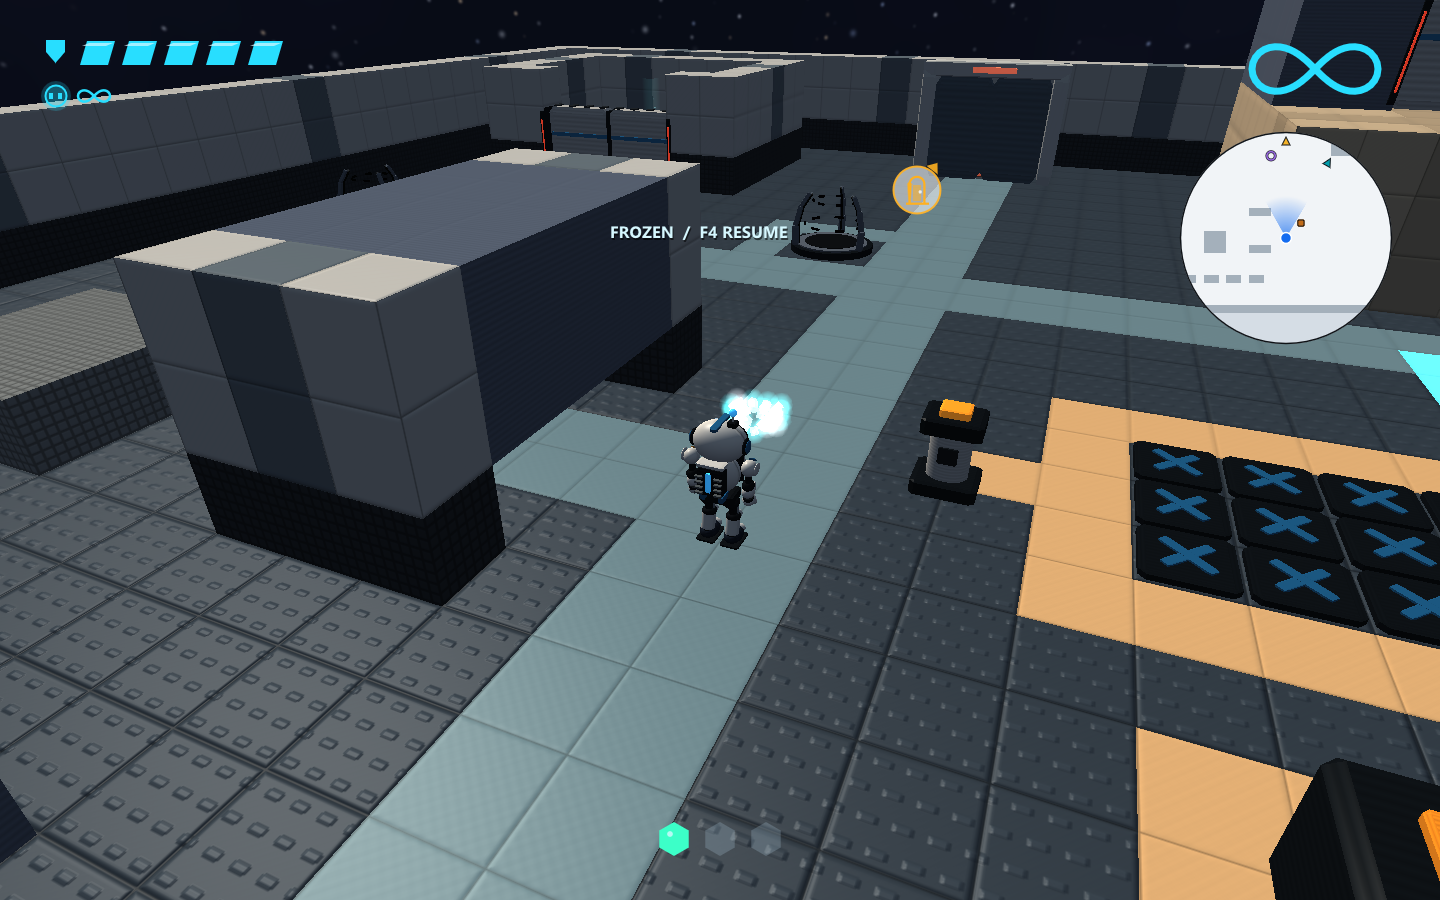
\includegraphics[width=\linewidth,trim=460bp 80bp 380bp 300bp,clip]{core.png}\par\small\textbf{(a) Core: 20 live particles}\end{minipage}\hfill
\begin{minipage}[t]{.32\linewidth}\centering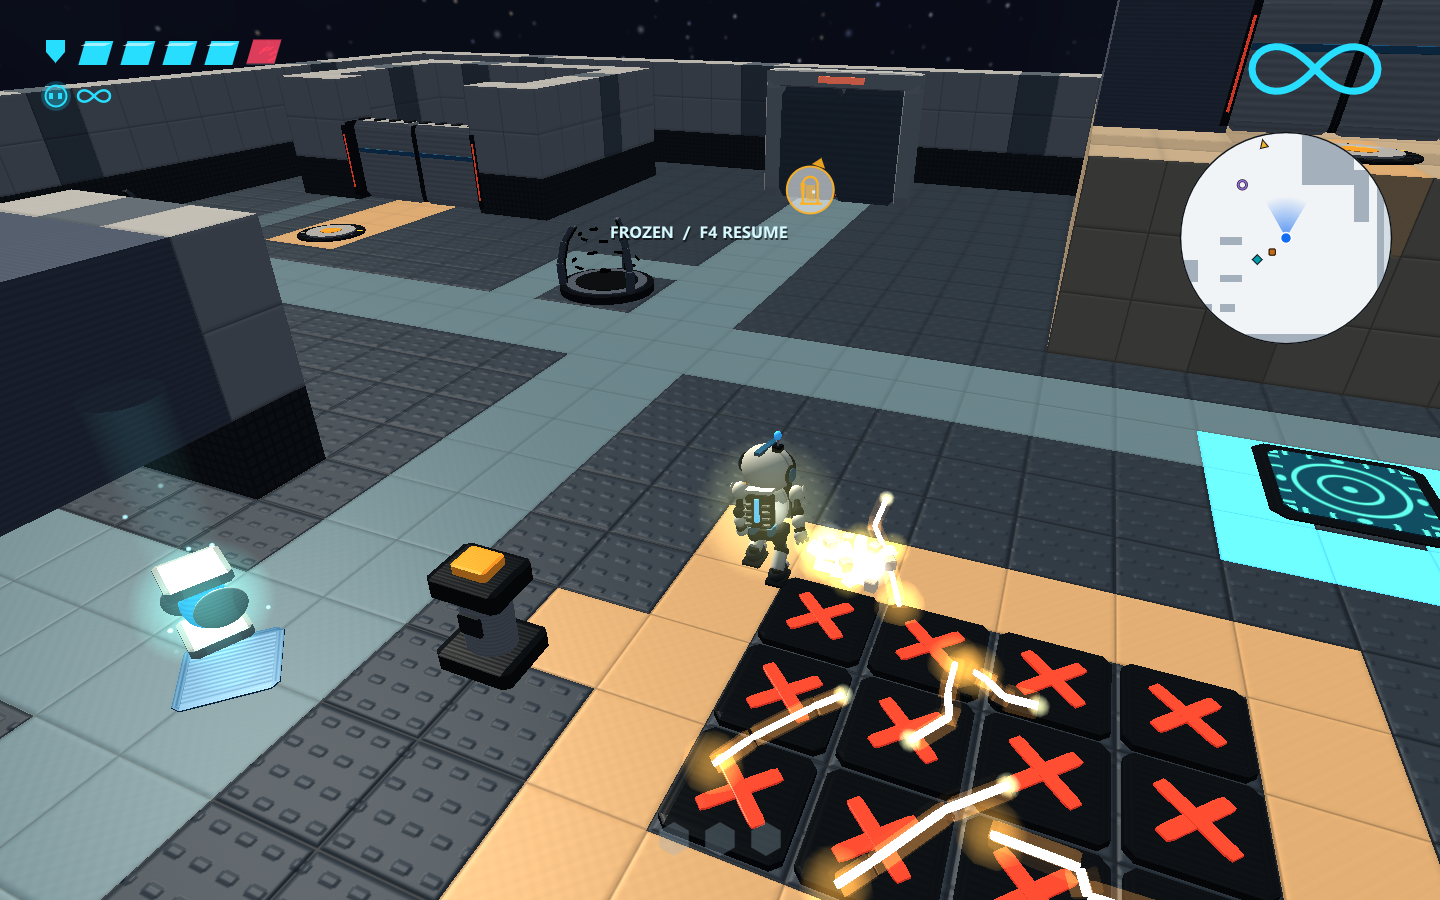
\includegraphics[width=\linewidth,trim=460bp 80bp 380bp 300bp,clip]{impact.png}\par\small\textbf{(b) Impact: 24 live particles}\end{minipage}\hfill
\begin{minipage}[t]{.32\linewidth}\centering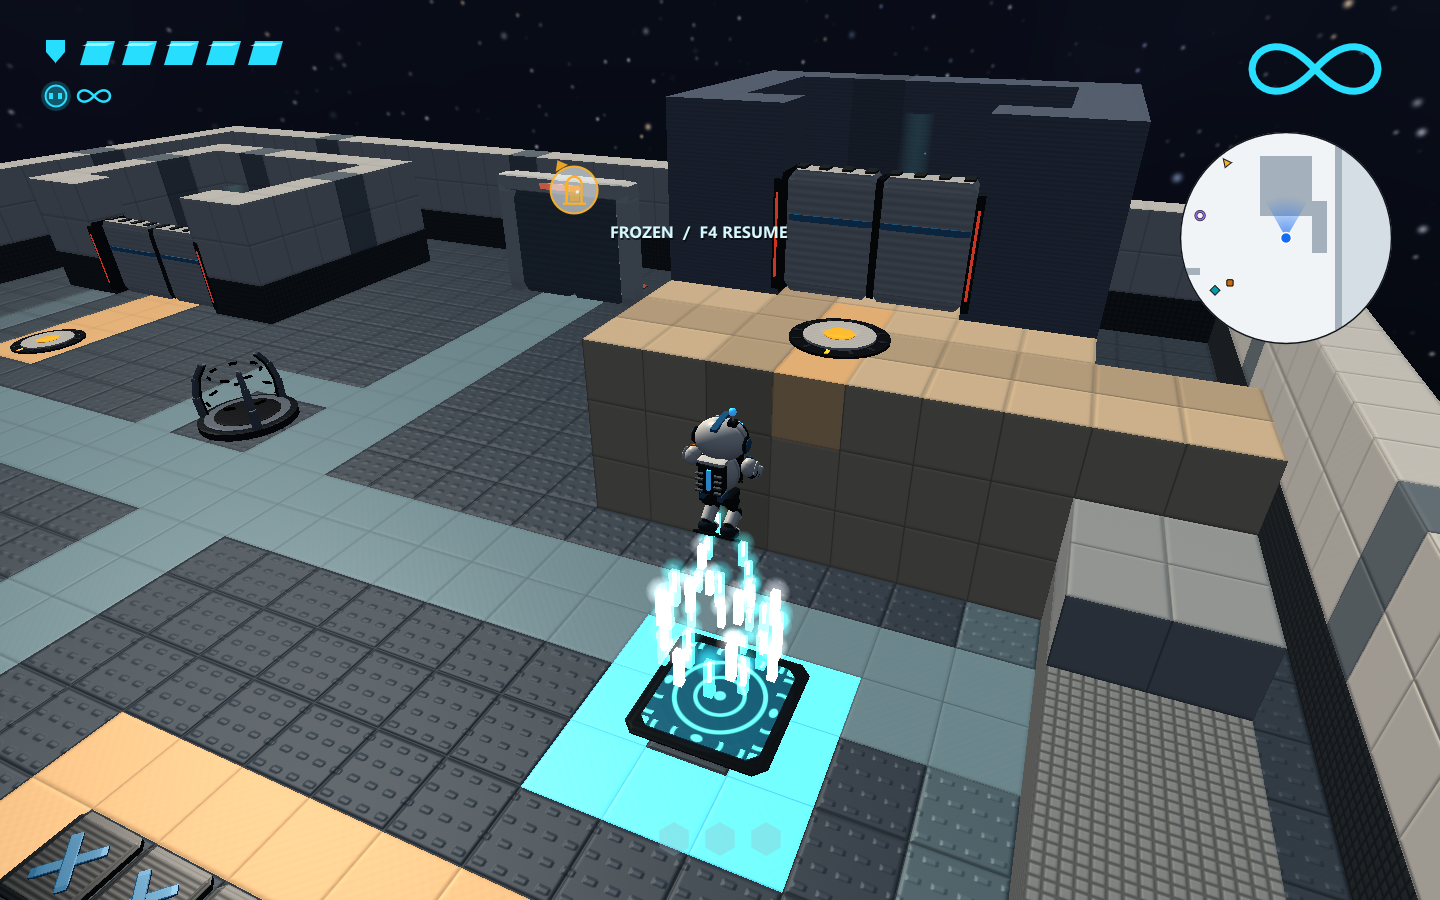
\includegraphics[width=\linewidth,trim=460bp 80bp 380bp 300bp,clip]{pad.png}\par\small\textbf{(c) Pad: 35 live particles}\end{minipage}
\caption{Detail crops from actual event captures (\code{-{}-effect core}, \code{impact}, \code{pad}); counts are the capture logs, not the maximum pool size. The pad count includes already-emitted trail particles.}\label{fig:particles}
\end{figure*}

\subsection{Purposeful hierarchical animation}
\code{CourierPose} poses the skeleton from movement and interaction state. Gait phases coordinate hip, knee and ankle rotation, with arm swing and torso motion; sprinting changes cadence and stride. Crouching lowers the pose, while jump, impact and shutdown states provide distinct feedback. Squash/stretch and body hop are visual offsets around the feet. The exit gate translates its two child panels when all cores are collected. Local animation therefore remains independent of the object's root position and orientation; it is procedural animation rather than a rigid-body ragdoll (Figure~\ref{fig:poses}).

\begin{figure*}[t]
\centering
\begin{minipage}[t]{.32\linewidth}\centering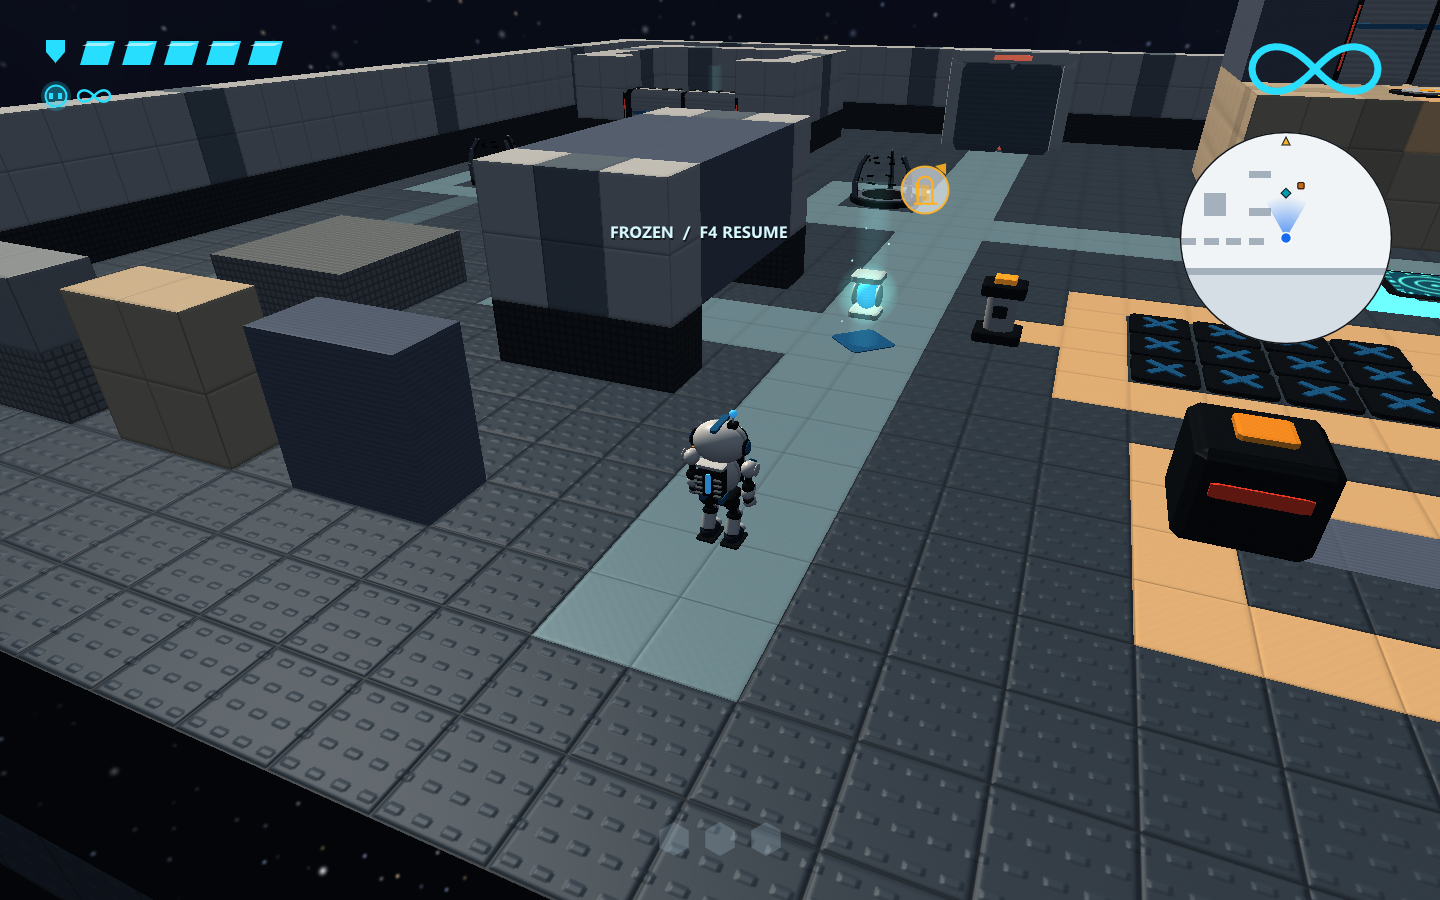
\includegraphics[width=\linewidth,trim=600bp 320bp 600bp 370bp,clip]{normal-on.png}\par\small\textbf{Standing}\end{minipage}\hfill
\begin{minipage}[t]{.32\linewidth}\centering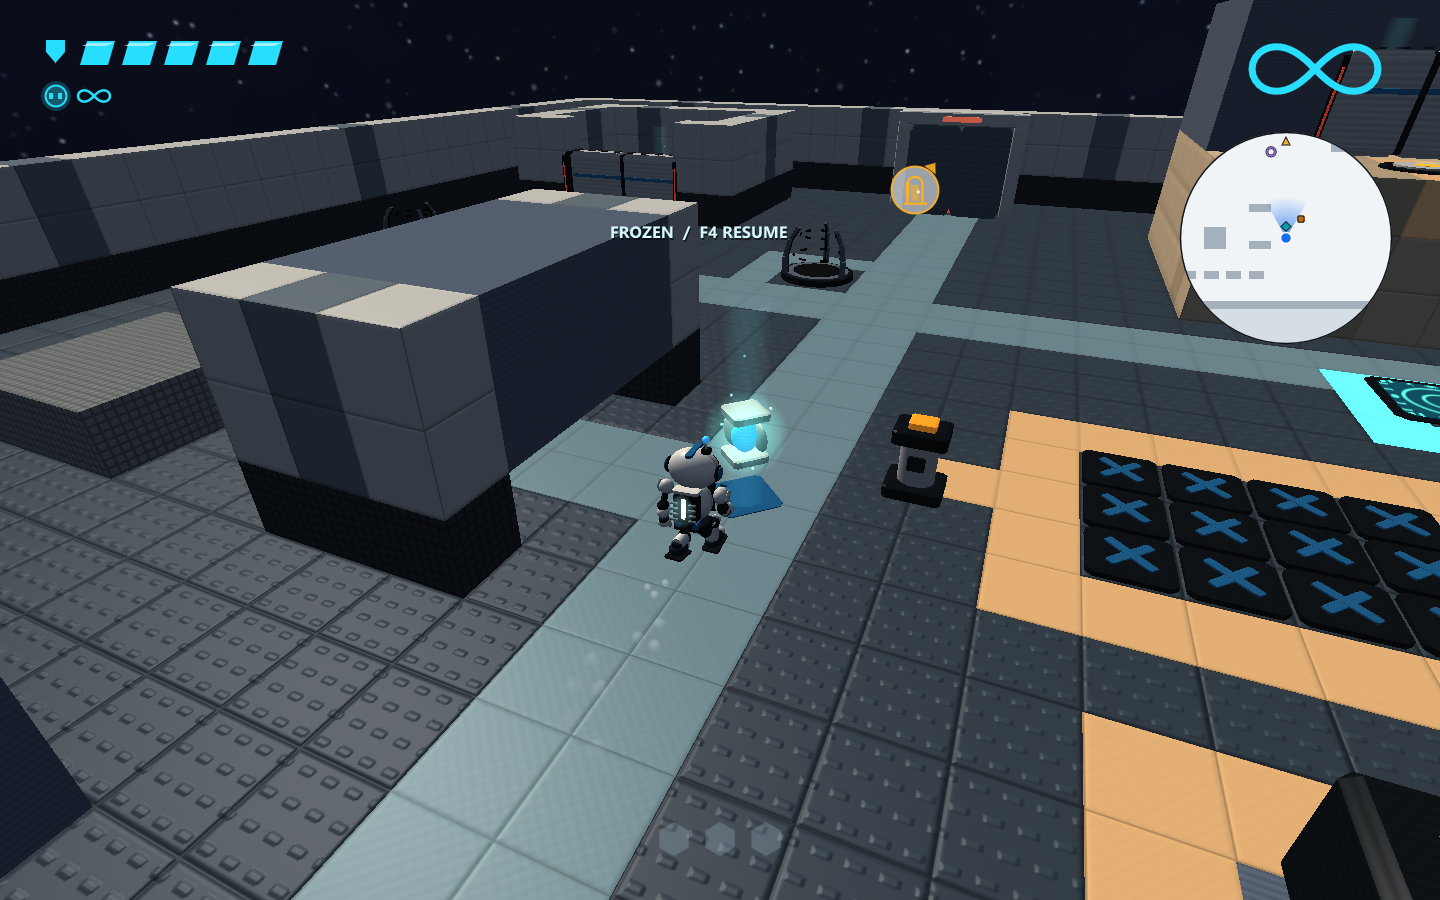
\includegraphics[width=\linewidth,trim=590bp 310bp 610bp 380bp,clip]{run.png}\par\small\textbf{Running}\end{minipage}\hfill
\begin{minipage}[t]{.32\linewidth}\centering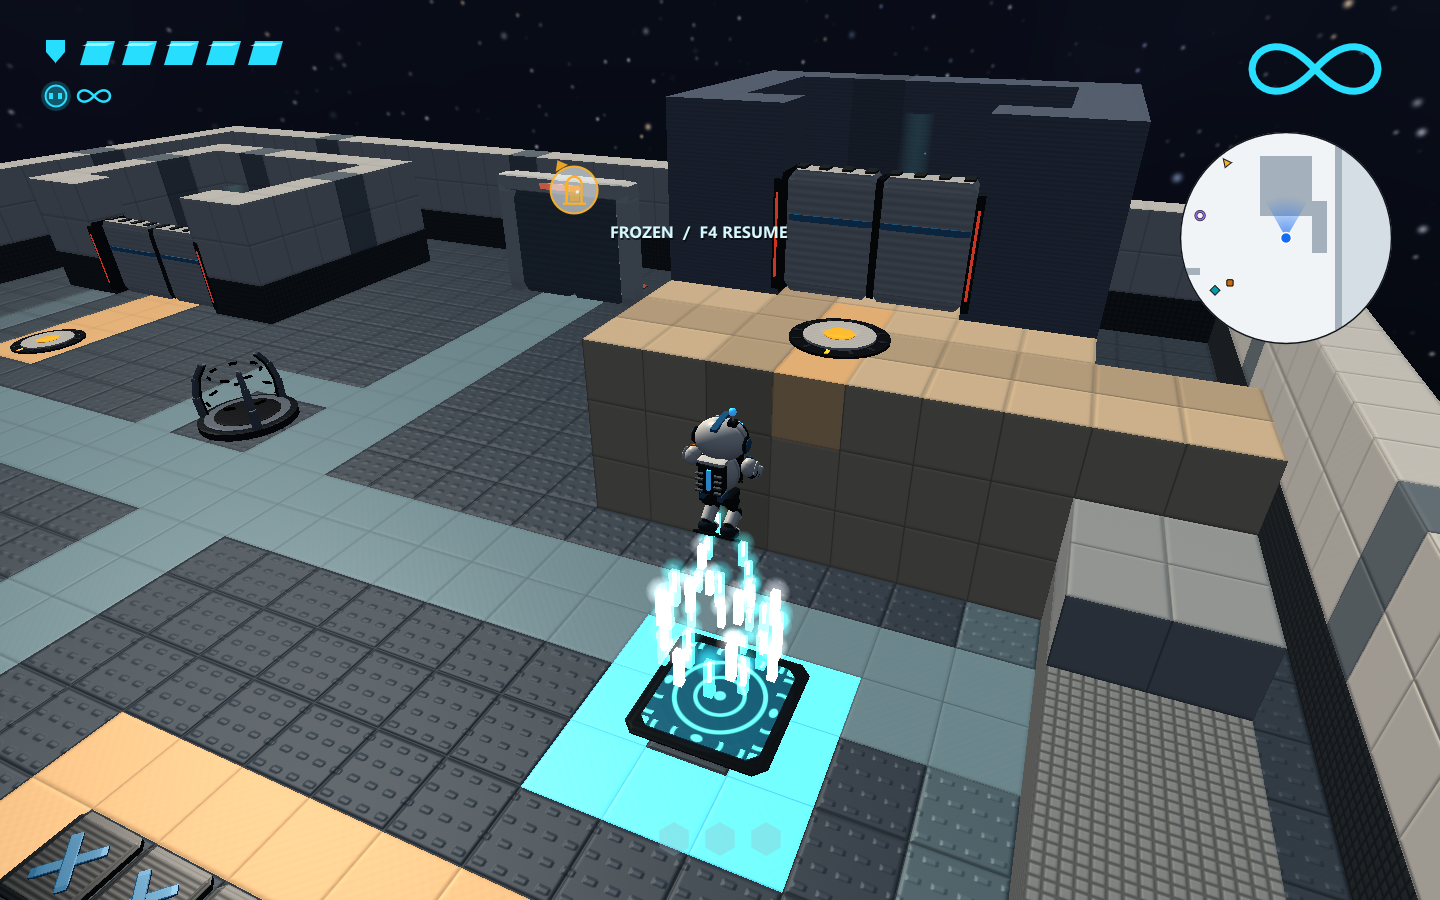
\includegraphics[width=\linewidth,trim=600bp 300bp 600bp 390bp,clip]{pad.png}\par\small\textbf{Pad ascent}\end{minipage}
\caption{Contrasting robot poses, enlarged from gameplay captures. Different joint angles, body height and limb placement make locomotion state visible.}\label{fig:poses}
\end{figure*}

\subsection{Validation boundary}
The event captures completed without reported OpenGL errors and showed the expected particle counts; the impact capture also reduced armour from five to four. Tests cover movement, damage cooldown, particle motion/recycling, restart state and pad emission. However, the gameplay test executable stops at a later Helios layout assertion, and route validation is incomplete (Section~\ref{sec:eval}). These observations support specific mechanisms, not a claim that every mission can currently be completed.


\section{Experimental Evaluation}\label{sec:eval}
\subsection{Controlled comparison}
The core optimisation removes a voxel face when its neighbouring cell is occupied. The baseline emits all six faces of every solid voxel. Both modes use the same instance grouping, shaders and effects; hidden-face removal is the only changed variable and is not counted again as an acceleration challenge. F6 toggles this optimisation interactively. Static terrain is rebuilt when the world revision or mode changes, outside the timed boundary.

Measurements were collected on 12 November using a Windows Release build (GCC 16.2.0), NVIDIA GeForce RTX 4060 Laptop GPU, driver 621.01, OpenGL 3.3. Each run used a \textbf{1920$\times$1080 framebuffer}, VSync off, \textbf{60 unmeasured warm-up frames} and \textbf{exactly 240 measured scene-render frames}. Each mode was repeated three times, alternating order. Table~\ref{tab:perf} averages those three 240-frame arithmetic means; every row has equal weight.

All scenes use the $96^3$ world and their fixed authored level files (no layout generation seed). The player is placed on the first jump pad, simulated for $24\times1/120=0.2$ seconds, then frozen with 35 active particles. The camera is at $(20,17,38)$, looking at $(20,1,19)$ with up $(0,1,0)$; vertical FOV is $50^\circ$, near/far planes 0.1/300. Normal mapping is ON at strength 1; the procedural sky and all prepared scene effects are included with render time fixed at zero. The same camera is retained across modes and levels; it samples a fixed view, not an entire play-through.

\begin{table*}[t]
\centering
\caption{Current-snapshot scene-rendering results. Reduction is $100(1-t_{opt}/t_{base})$. Counts include terrain, model instances, effects and the sky triangle.}\label{tab:perf}
\small
\begin{tabular}{@{}lrrrll@{}}\toprule
&\multicolumn{2}{c}{\textbf{Mean ms/frame}}&&&\\
\textbf{Scene} & \textbf{Base} & \textbf{Opt.} & \textbf{Reduction} & \textbf{Triangles: base $\to$ opt.} & \textbf{Draws}\\\midrule
Tutorial & 2.606 & 2.395 & 8.1\% & 93,129 $\to$ 77,493 & 9 $\to$ 9\\
Helios & 3.019 & 2.470 & 18.2\% & 380,137 $\to$ 222,713 & 10 $\to$ 10\\
Corona & 2.929 & 2.353 & 19.7\% & 321,017 $\to$ 170,173 & 10 $\to$ 10\\\bottomrule
\end{tabular}
\end{table*}

\textbf{Interpretation.} Triangle counts decrease by 16.8\%, 41.4\% and 47.0\%, respectively. Draw-call counts are unchanged because culling reduces the terrain mesh, not the number of material/instance batches. Timing gains are smaller than geometry reductions: sky shading, other fragments and fixed draw overhead remain. Across repeats, baseline/optimised ranges were 2.549--2.635/2.369--2.426 ms (Tutorial), 2.950--3.154/2.467--2.475 ms (Helios), and 2.851--3.080/2.339--2.377 ms (Corona). These are local observations, not cross-device guarantees.

\textbf{Timing boundary and image checks.} \code{glFinish} drains previous work before the CPU timer and waits for scene completion before stopping it. Thus the result includes scene submission and completion, not a pure GPU timestamp. Loading, mesh preparation, simulation, ImGui, screenshot capture and buffer swapping are excluded. First-pair baseline/optimised screenshots differed in fewer than 0.005\% of pixels, with mean absolute RGB error below 0.002 on the 0--255 scale; they are nearly, but not exactly, identical. Exact CSVs and source fingerprints accompany the editable report.

\textbf{Reproduction.} The benchmark is invoked from the repository root using \code{-{}-benchmark}, \code{-{}-level 0} and \code{-{}-benchmark-output tutorial.csv}. Levels 1 and 2 select Helios and Corona, respectively. The executable performs all six measurements per level and saves the first baseline/optimised image pair. Use the current source and level files: the November 7 binary and older benchmark tables describe different scenes.

\subsection{Current validation status}
The Windows game and five game-test targets build successfully. Of six registered CTest suites, tutorial and surveillance-camera suites pass. The editor and Corona suites expect ten Corona cores (now nine), and the Corona suite also expects at least eight movers (now six); the gameplay suite expects six Helios doors/plates (now five); the Helios route search cannot reach the indexed west inner plate. This leaves three game suites plus the editor suite failing. These failures require map/test reconciliation and route revalidation. A successful VLAB/CSE build and play-through has not yet been established for this snapshot.


\section{Contributions and Discussion}\label{sec:discussion}
\subsection{Responsibilities and integration}
\textbf{Jacky Hui is Member A, and Jerry Xie is Member B.} Their responsibilities follow the division established in the revised project plan. \textbf{Member A (Jacky Hui)} covers player movement and interactions, hazards, lives/checkpoints, training, controls and menus, robot animation, gameplay feedback and particle lifecycle. \textbf{Member B (Jerry Xie)} covers voxel terrain and level layouts, materials and lighting, normal mapping, environment rendering, optimisation measurement and the planned VLAB/CSE validation. Both roles meet at mechanism placement, scene state, camera behaviour, regression testing and the demonstration.

Relevant history includes \code{53a3ba9} (jump-pad plume/trail), \code{8ae7ec6} (five procedural materials), \code{8909214} (normal/particle demonstrations and benchmarks), and \code{1af555e} (tutorial, Corona and reboot integration). Jerry's \code{735305f} adds the minimap and mouse-linked facing; \code{e71999d} documents its integration. These commits locate feature/integration evidence; the responsibility split is not a claim that each commit has the corresponding member as its sole author. Measurements include local changes after \code{1af555e}.

\subsection{Individual technical reflections}
\textbf{Member A (Jacky Hui).} The main lesson in the gameplay role is to separate presentation from authoritative simulation state. Limb animation and recoil should communicate movement without moving the collision body through walls. Death, reboot, pause and full restart also need different reset rules: retaining cores during recovery must not retain them after a new run. Event captures help inspect this feedback, while state-based tests are needed to check timers, cooldowns and particle cleanup. The remaining route failures show why visible local mechanisms are insufficient evidence of a complete playable mission.

\textbf{Member B (Jerry Xie).} The rendering role highlights the importance of consistent coordinate spaces and controlled comparisons. A normal map needs a correct UV basis, especially on scaled and curved parts; extra texture detail alone does not establish correctness. Hidden-face removal substantially reduces submitted triangles, but scene time also depends on shader and fixed costs. Level-file edits must be reconciled with mechanism indices and route tests before freezing the final scenes. The outstanding platform check remains an essential part of this role's planned delivery.

\subsection{Comparison with the Project Plan} The two selected challenges remain Normal Mapping and Particles. The implementation replaces the earlier courtyard/corridor missions with Helios and Corona, grows storage from $64^3$ to $96^3$, reduces the particle pool from 1,024 to 128, and uses a procedural sky. Optional power-ups/speed pads from the plan are outside the current authored levels. Reboot timing and progression rules have also changed. Final-stage priorities are resolving map/test mismatches, validating complete routes on VLAB/CSE, and refreshing evidence after changes.


\subsection{External Software and Assets}
The project extends the course starter's window, shader and UI foundation. CMake \code{FetchContent} integrates GLFW for window/context management and input~\cite{glfw}, GLAD for OpenGL function loading~\cite{glad}, GLM for vector and matrix mathematics~\cite{glm}, Dear ImGui and its GLFW/OpenGL backends for the interface~\cite{imgui}, and stb for image input/output~\cite{stb}. The evaluated build uses existing local dependency overrides; declared versions and licence sources are provided in the references.

Geometry, material textures and the current star sky are generated by project code; no external model or sky photograph is used in the reported captures. The bundled Rajdhani SemiBold font is distributed under SIL OFL 1.1~\cite{rajdhani}. On Windows, the application may instead load Segoe UI Bold from the installed system; its font file is not redistributed with the project~\cite{segoe}.

\section{Conclusion}
Core Explorer integrates voxel collision, articulated modelling, material shading and event-driven feedback within three distinct configurations. The controlled benchmark shows that removing internal voxel faces reduces submitted triangles and scene-rendering time, while substantial shader and fixed rendering costs remain. Normal-map comparisons and event captures provide evidence for the two selected challenge tasks. Complete-route validation, reconciliation of map-dependent tests and verification on VLAB/CSE remain necessary before the evaluated development version can be treated as a final submission.

\balance
\begin{thebibliography}{7}
\small
\setlength{\itemsep}{2pt plus 1pt minus 1pt}
\bibitem{glfw}
GLFW Development Team, \textit{GLFW 3.3.10}, zlib/libpng licence. [Online]. Available: \url{https://github.com/glfw/glfw/blob/3.3.10/LICENSE.md}.
\bibitem{glad}
D. Herberth, \textit{GLAD 2.0.8}, MIT licence; additional Khronos terms for specifications. [Online]. Available: \url{https://github.com/dav1dde/glad/blob/v2.0.8/LICENSE}.
\bibitem{glm}
G-Truc Creation, \textit{OpenGL Mathematics (GLM) 1.0.3}, MIT or Happy Bunny licence. [Online]. Available: \url{https://github.com/g-truc/glm/blob/1.0.3/copying.txt}.
\bibitem{imgui}
O. Cornut, \textit{Dear ImGui 1.92.9b}, MIT licence. [Online]. Available: \url{https://github.com/ocornut/imgui/blob/v1.92.9b/LICENSE.txt}.
\bibitem{stb}
stb contributors, \textit{stb}, commit \code{2c980bb}, MIT or public-domain alternative. [Online]. Available: \url{https://github.com/nothings/stb/blob/2c980bb59875b0d32144a71867fbdebb2f77cd20/LICENSE}.
\bibitem{rajdhani}
Indian Type Foundry, \textit{Rajdhani}, SIL Open Font License 1.1, 2014. [Online]. Available: \url{https://github.com/google/fonts/tree/main/ofl/rajdhani}. Licence retained in \path{assets/fonts/OFL-Rajdhani.txt}.
\bibitem{segoe}
Microsoft, \textit{Segoe UI font family}, installed Windows font; separate terms apply to redistribution. [Online]. Available: \url{https://learn.microsoft.com/en-us/typography/font-list/segoe-ui}.
\end{thebibliography}
\end{document}
